\section{Methodology}
\label{sec:methodology}

DynSTEER establishes a dynamic evaluation framework for agent trajectory, as illustrated in Figure~\ref{fig:overall_framework}. Rather than treating rollouts as opaque black boxes or enforcing rigid single-path matching, DynSTEER coordinates three core components: stage-wise dynamic evaluation to resolve the evidence-granularity problem, which Sections~\ref{sec:stage_alignment} and~\ref{sec:routing_early_stop} present; path-tolerant milestone-graph generation to preserve execution diversity, which Section~\ref{sec:blueprint_compilation} presents; and execution-time early termination to curb resource waste, which Section~\ref{sec:routing_early_stop} presents.

\begin{figure*}[t]
\centering
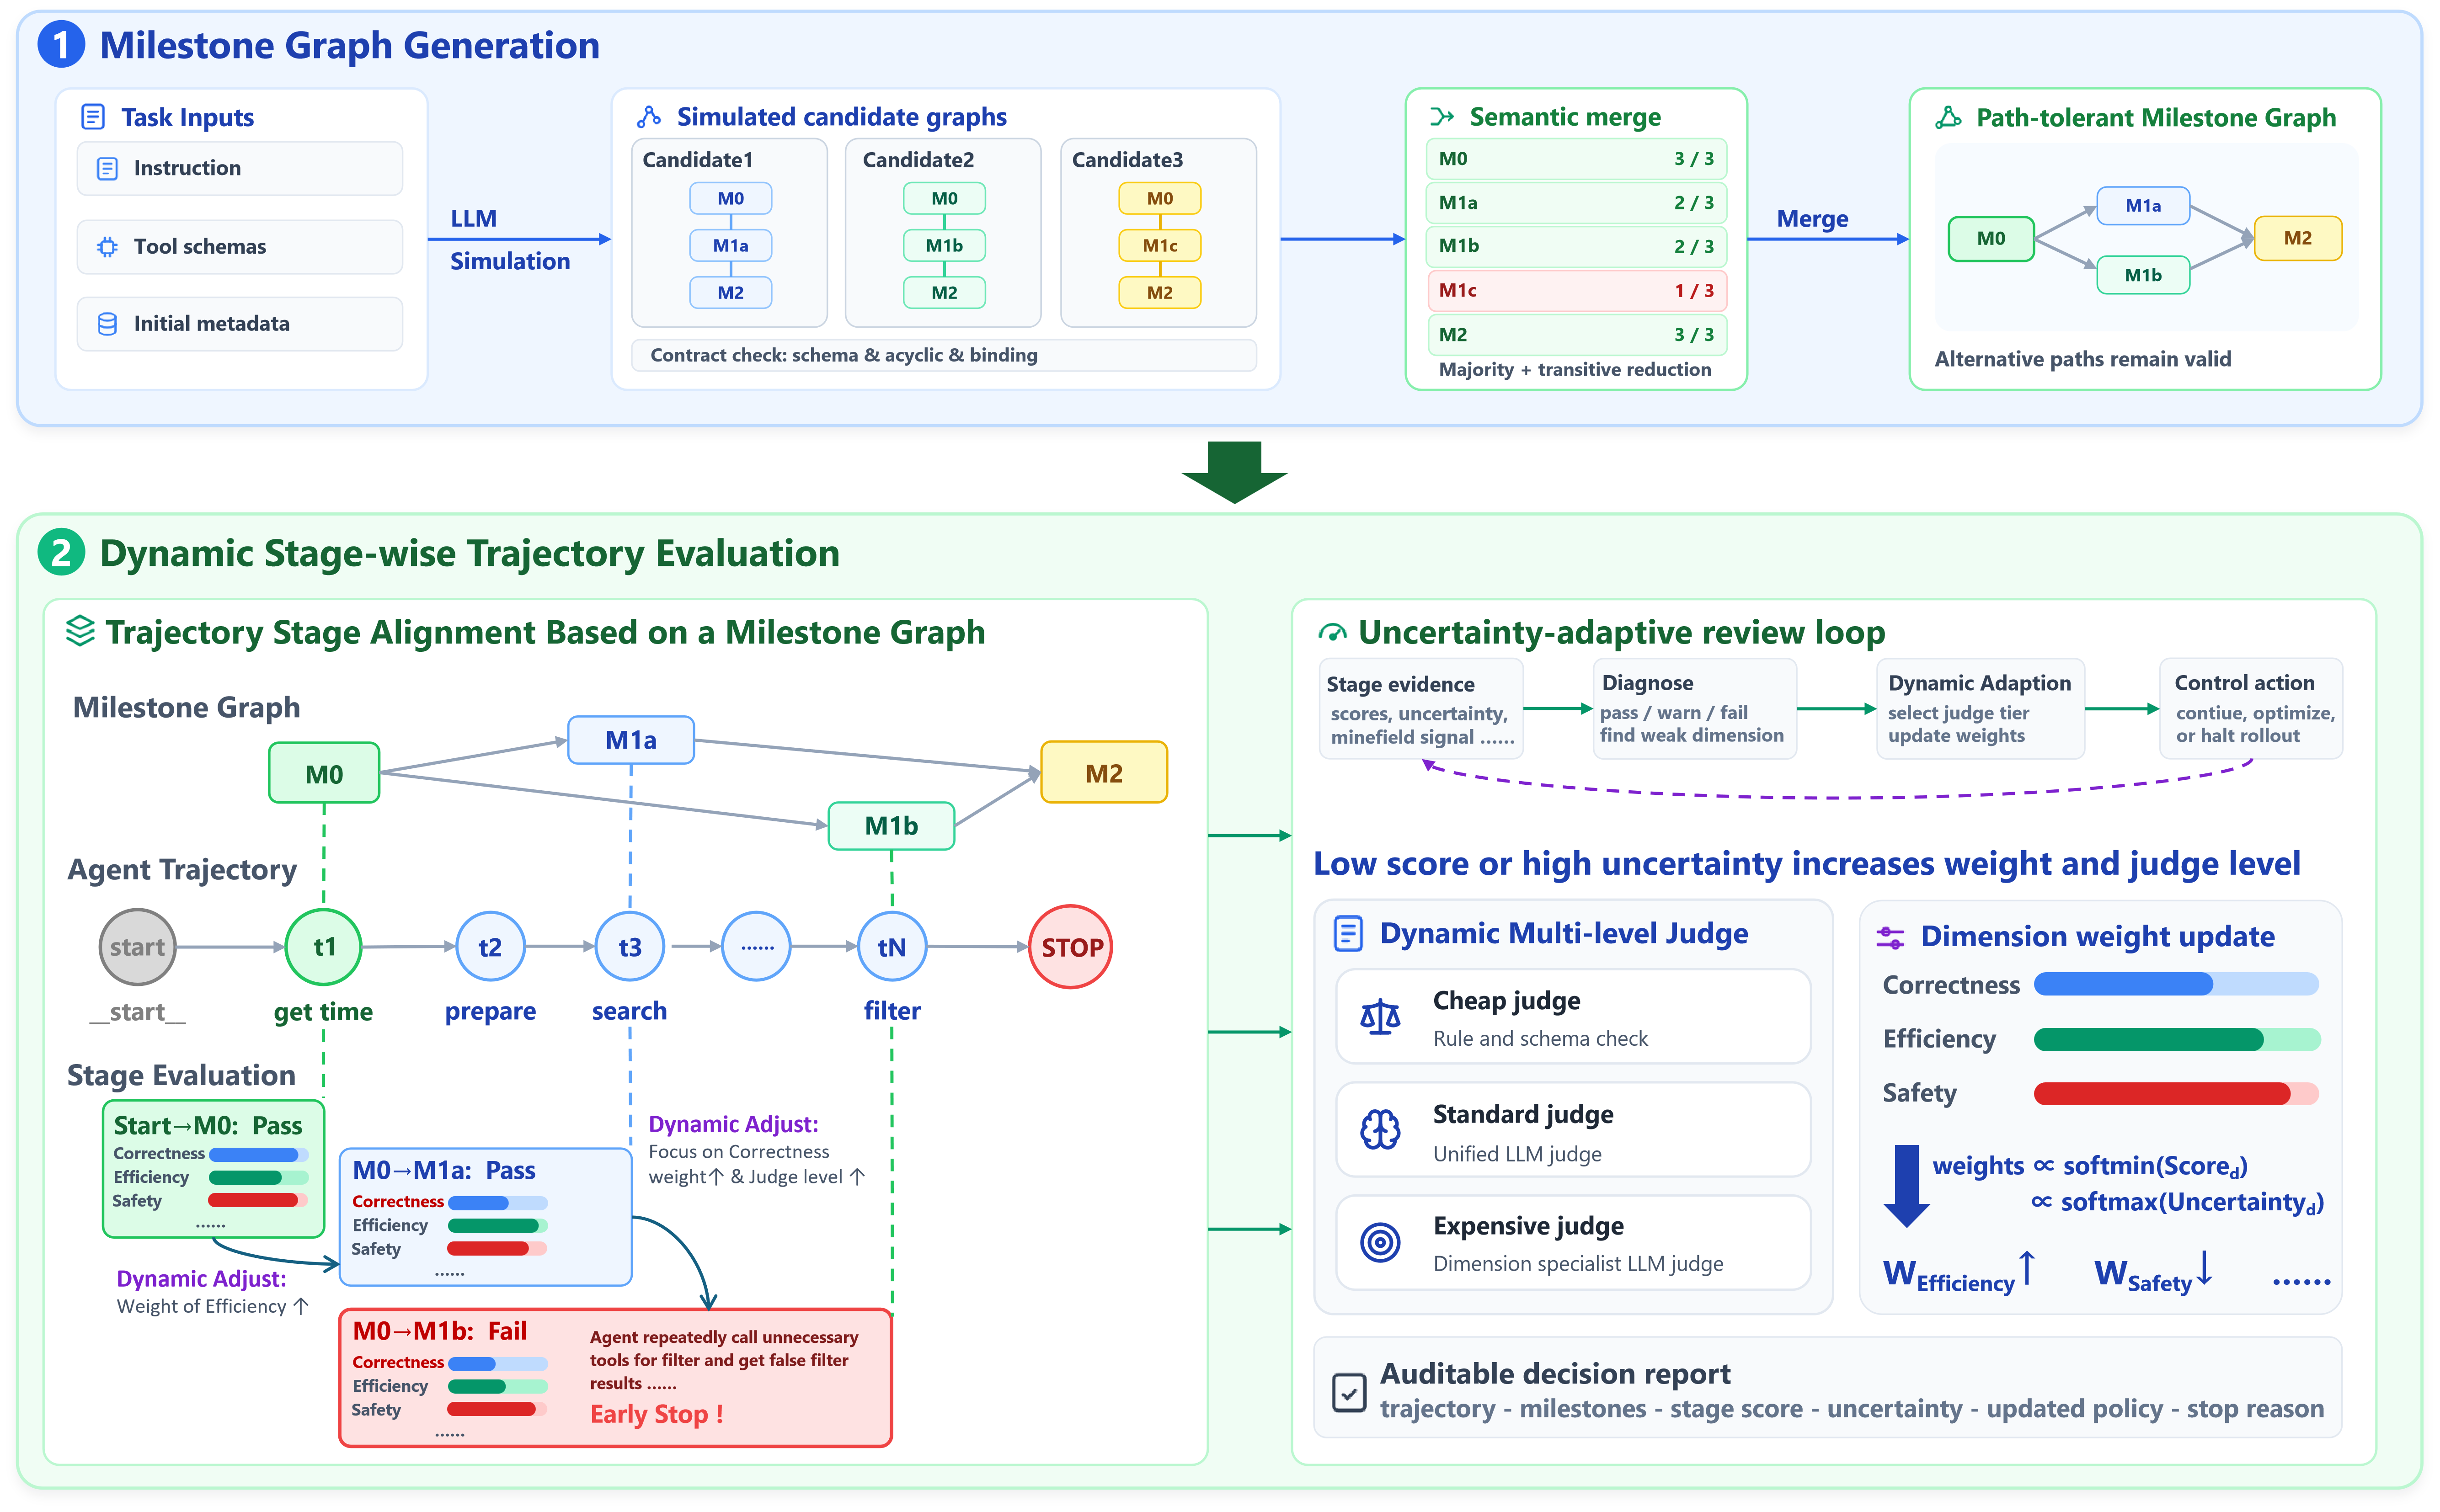
\includegraphics[width=0.96\textwidth]{figures/overall-framework.png}
\vspace{-0.25cm}
\caption{\textbf{Overview of the \textsc{DynSTEER} Workflow.} (1) Pre-execution milestone graph generation synthesizes multi-candidate simulated rollouts from task inputs to compile a path-tolerant DAG. (2) Execution-time stage-wise evaluation aligns closed actions, isolates dominator evidence windows to evaluate weak links with trajectory context, adaptively scales judge levels, and records executable early-stop decisions for subsequent evaluation control.}
\label{fig:overall_framework}
\vspace{-0.35cm}
\end{figure*}

\subsection{Task Inputs and Dual-Clock Observation}
\label{sec:formulation}
Following interactive tool-using agent environments~\citep{gu2024toolsandbox,yang2023intercode,liu2023agentbench}, a task provides instruction $x$, initial state $\mathcal{S}_0$, API catalog $\mathcal{A}$, and safety contracts $\mathcal{C}$. DynSTEER evaluates the task inputs
\begin{equation}
    V_{\text{task}} = (x, \mathcal{A}, \mathcal{I}_0),
    \label{eq:task_inputs}
\end{equation}
where $\mathcal{I}_0$ is evaluator-visible initial-state metadata; hidden reference paths $\tau^*$ and terminal unit tests are never used for graph construction.

During execution, the trace $\tau = \langle e_1, \dots, e_K \rangle$ is observed on two clocks. 
The raw event clock $k$ indexes every observed event and triggers immediate fatal-action interception, whereas the closed-action clock $t$ advances only after a tool return is observed and the agent yields control. Milestone settlement and scoring use $t$. 
For example, in $\langle \text{tool call}, \text{tool return}, \text{agent yield} \rangle$, the three observations receive raw indices $k=1,2,3$, so a hazardous tool call can be intercepted at $k=1$. 
The action closes at $k=3$, where $t$ advances from $0$ to $1$ and becomes the unit used for milestone settlement. 
This dual-clock design couples safety responsiveness with semantic completeness: the raw event clock exposes fatal minefield operations as soon as the agent attempts them, whereas the closed-action clock prevents milestone settlement from missing information or state changes.

\subsection{Milestone Graph Generation via Simulated Planning}
\label{sec:blueprint_compilation}
To overcome single-reference bias, DynSTEER compiles $V_{\text{task}}$ into a path-tolerant Milestone Graph $G = (M, E, \mathcal{K}, \mathcal{M}_{\text{fatal}})$ prior to execution, where $M$ is the milestone set, $E$ encodes precedence constraints, $\mathcal{K}$ specifies parameter bindings, and $\mathcal{M}_{\text{fatal}}$ defines hazardous operations.

\textbf{Multi-Candidate Synthesis and Contract Validation.} Given $V_{\text{task}}$, a blueprint generator synthesizes $C$ candidate plans $\{G_1, \dots, G_C\}$ via LLM prompting across diverse exploration heuristics, such as direct keyword queries versus hierarchical filtering. Each candidate $G_c = (M_c, E_c)$ undergoes deterministic contract verification:
\begin{equation}
    \text{Valid}(G_c) = \text{SchemaCheck}(M_c, \mathcal{A}) \land \text{Acyclic}(E_c) \land \text{BindingConsistency}(\mathcal{K}_c)
    \label{eq:valid_gc}
\end{equation}
Here, SchemaCheck requires every milestone and minefield to name an available API and to match its argument and return schema; Acyclic rejects circular precedence constraints; BindingConsistency requires dynamic bindings to reference declared upstream outputs with compatible parameter types. A candidate failing any check is discarded. Appendix~\ref{app:contract_validation} details these deterministic filters.

\textbf{Strict-Majority Consensus and Transitive Reduction.} To retain essential invariants while preserving exploratory flexibility, a milestone $m$ is retained if and only if it appears in a strict majority of valid candidates:
\begin{equation}
    M = \left\{ m \;\middle|\; \sum_{c=1}^{C_{\text{valid}}} \mathbb{I}[m \in M_c] \ge \left\lceil \frac{C_{\text{valid}} + 1}{2} \right\rceil \right\}
    \label{eq:consensus}
\end{equation}
Precedence edges are aggregated analogously. Finally, we compute the transitive reduction $E = \text{TR}(E_{\text{majority}})$~\citep{tarjan1972depth} to eliminate redundant shortcut dependencies, producing a minimal directed acyclic graph that accommodates diverse legitimate execution strategies.

\subsection{Stage-wise Dynamic Trajectory Evaluation}
\label{sec:stage_alignment}
During execution, DynSTEER dynamically aligns closed actions against the milestone graph. Algorithm~\ref{alg:dynsteer} in Appendix~\ref{app:algorithms} presents the complete algorithmic flow.

\textbf{Ready Frontier Matching.} Let $M_{<t}$ denote milestones settled prior to closed action $t$. The active search space is strictly bounded by the \textbf{ready frontier}:
\begin{equation}
    \mathcal{F}_t = \{ m \in M \setminus M_{<t} \mid \text{Pred}(m) \subseteq M_{<t} \}
    \label{eq:frontier}
\end{equation}
An action $a_t$ settles milestone $m^* \in \mathcal{F}_t$ if its tool call and state delta satisfy semantic predicates $\phi_{m^*}(a_t, s_t) = 1$. Restricting alignment to $\mathcal{F}_t$ prevents out-of-order settlement and reward gaming.

\textbf{Dominator-Anchored Stage Isolation.} To construct a semantically complete stage evidence window for $m^*$, DynSTEER computes the immediate dominator $\text{idom}(m^*)$ in $G$~\citep{lengauer1979fast}, defined as the unique node that must be traversed on every directed path from start node $s_0$ to $m^*$. The \textbf{stage evidence window} is bounded by:
\begin{equation}
    \mathcal{W}(m^*) = [t_{\text{idom}(m^*)}, t]
    \label{eq:stage_window}
\end{equation}
where $t_{\text{idom}(m^*)}$ is the execution step at which the dominator was settled. 
Anchoring evidence to $\mathcal{W}(m^*)$ preserves all intermediate reasoning, trial-and-error attempts, and parameter adjustments that lead directly to $m^*$, ensuring that relevant actions are not omitted merely because the agent executes them in parallel branches.
Unlike whole-trajectory evaluation, which obscures mistake locations, and single-step evaluation, which lacks context, dominator-anchored stages provide enough trajectory context to evaluate intermediate quality and pinpoint the exact first-error step.

\textbf{Multidimensional Scoring.} DynSTEER scores the entire evidence window $\mathcal{W}(m^*)$. Each stage uses a task-relevant subset $\mathcal{D}_t \subseteq \mathcal{D}$ of seven dimensions: progress, state consistency, tool quality, efficiency, safety, interaction quality, and recovery. The composite stage score is:
\begin{equation}
    S_t = \sum_{d \in \mathcal{D}} w_d^{(t)} s_d^{(t)}(m^*)
    \label{eq:stage_scoring}
\end{equation}
parameterized by dynamically normalized weights $\mathbf{w}^{(t)}$.
Uncertainty-adaptive multi-level review then treats these stage scores and uncertainty estimates as control signals, allocating stronger review capacity to ambiguous or weak dimensions. 

\subsection{Uncertainty-Adaptive Review and Execution-Time Early Termination}
\label{sec:routing_early_stop}
Uncertainty-adaptive review is the control layer for stage-wise evaluation, adjusting dimension weights and judge levels after each stage. 
Execution-time early termination is a separate downstream safeguard that reuses the same stage evidence to control resource waste.

\textbf{Multi-Level Judge Structure.} Rather than assigning a uniform evaluator across all stages, DynSTEER deploys a three-level judge hierarchy whose prompt templates are detailed in Appendix~\ref{app:prompts}:
\begin{itemize}[leftmargin=*,itemsep=1.5pt,topsep=1pt]
    \item \textbf{Level 1: Cheap Judge} ($J_{\text{cheap})}$: A deterministic structural evaluator inspecting tool status codes, schemas, and evidence rules without LLMs, incurring zero model inference overhead.
    \item \textbf{Level 2: Standard Judge} ($J_{\text{std})}$: A multi-field unified LLM evaluator scoring all target dimensions simultaneously within a single pass, aggregating confidence across multiple samples.
    \item \textbf{Level 3: Expensive Judge} ($J_{\text{exp})}$: A single-dimension specialist LLM evaluator executing dedicated expert rubrics and deep counterfactual analysis across multiple deliberation passes to capture subtle behavioral defects.
\end{itemize}

\textbf{Uncertainty-Adaptive Review Adjustment.} DynSTEER dynamically shifts evaluation weights and escalates judge levels toward an agent's vulnerable links. First, dimension weights are updated via exponential gradient scaling:
\begin{equation}
    w_d^{(t+1)} = \frac{w_d^{(t)} \cdot \exp\left( \alpha (1 - s_d^{(t)}) + \beta u_d^{(t)} \right)}{\sum_{d' \in \mathcal{D}} w_{d'}^{(t)} \cdot \exp\left( \alpha (1 - s_{d'}^{(t)}) + \beta u_{d'}^{(t)} \right)}
    \label{eq:weight_update}
\end{equation}
where $s_d^{(t)} \in [0, 1]$ is the dimension score, $u_d^{(t)} \in [0, 1]$ is dimension uncertainty, and $\alpha, \beta$ scale sensitivity to quality deficits and uncertainty. Appendix~\ref{app:weighting_rationale} gives the design rationale and mathematical derivation of this update. Second, dimensions with low scores or high uncertainty receive increased attention in the next-stage evaluation, which is formalized as follows: the baseline judge level is:
\begin{equation}
    \text{Level}_{\text{base}}^{(t+1)} =
    \begin{cases}
    J_{\text{cheap}}, & \text{if } S_t \ge \theta_{\text{pass}} \;\land\; \max_{d} u_d^{(t)} \le \theta_{\text{low\_u}} \;\land\; \mathcal{M}_{\text{fatal}}^{(t)} = 0 \\
    J_{\text{std}}, & \text{otherwise}
    \end{cases}
    \label{eq:level_base}
\end{equation}
For each individual dimension $d$, its level $\text{Level}_d^{(t+1)}$ adaptively escalates along $J_{\text{cheap}} < J_{\text{std}} < J_{\text{exp}}$:
\begin{equation}
    \text{Level}_d^{(t+1)} =
    \begin{cases}
    J_{\text{exp}}, & \text{if } s_d^{(t)} < \theta_{\text{fail}} \\
    \min\left(J_{\text{exp}},\, \text{Level}_d^{(t)} + 1\right), & \text{if } s_d^{(t)} < \theta_{\text{warn}} \lor u_d^{(t)} \ge \theta_{\text{high\_u}} \\
    \text{Level}_{\text{base}}^{(t+1)}, & \text{otherwise}
    \end{cases}
    \label{eq:level_dim}
\end{equation}
This focuses expensive LLM deliberation selectively on weak or ambiguous execution links while relaxing confident stages to rule-based verification to minimize unnecessary LLM invocations.
Together with stage segmentation and local evidence isolation, this evaluation strategy resolves the evidence-granularity problem. 
% The next mechanism addresses a distinct objective: preventing unrecoverable prefixes from consuming further execution resources.

\textbf{Execution-Time Early Termination.} To prevent runaway executions on unrecoverable trajectories, DynSTEER monitors three policy stopping criteria.
First, \textbf{Fatal Minefield Interception}, where $e_k \in \mathcal{M}_{\text{fatal}}$, signals immediately on the raw event clock upon hazardous or irreversible actions.
Second, \textbf{Persistent Low Quality}, where $S_t < \theta_{\text{fail}}$, signals when accumulated stage deficits indicate unrecoverable goal drift.
Third, \textbf{Frontier Stagnation} signals when an agent takes $N_{\text{stag}}$ consecutive actions without advancing the ready frontier $\mathcal{F}_t$, detecting pathological loops.
A stop emits an auditable report recording the step, dominator anchor, and causal failure dimension.
In our controlled experiments, we replay the decision against a complete source trajectory: the report defines a virtual stop boundary, and we measure efficiency by matching that boundary to the recorded prefix of the source execution.